\documentclass[12pt]{article}
\usepackage{amsmath,amsfonts,fullpage,amsthm,graphicx}

\newtheorem*{theorem}{Theorem}
\newtheorem*{fact}{Fact}
\newtheorem*{goal}{Goal}
\newtheorem*{idea}{Idea}
\newtheorem*{defn}{Definition}
\newtheorem*{ex}{Example}

%Style section
%\setlength{\textheight}{10in}
%\setlength{\textwidth}{7in}
%\hoffset=-0.75in
 \pagestyle{plain}
% \setlength{\topmargin}{0in}
% \setlength{\headsep}{0in}
% \setlength{\oddsidemargin}{0in}
% \setlength{\evensidemargin}{0in}

\begin{document}


\pagestyle{empty} %use this to get rid of page numbers

\noindent
{Math 166 \hskip 1.5 truein  Names:\ \hrulefill}

\noindent
%\vskip 0.3truein
%\bigskip
%\noindent
{Integration strategies}

\noindent  \hskip 3.5 truein  Section Number:\ \hrulefill
\medskip

\begin{goal} \rm
Evaluate the following integrals by any method
\end{goal}
%\smallskip

\begin{enumerate}
%\setcounter{enumi}{-1}
%\item (Review)
%Write an expression for each of the six trig functions in terms of the lengths of the sides of the right triangle below:

%\medskip
%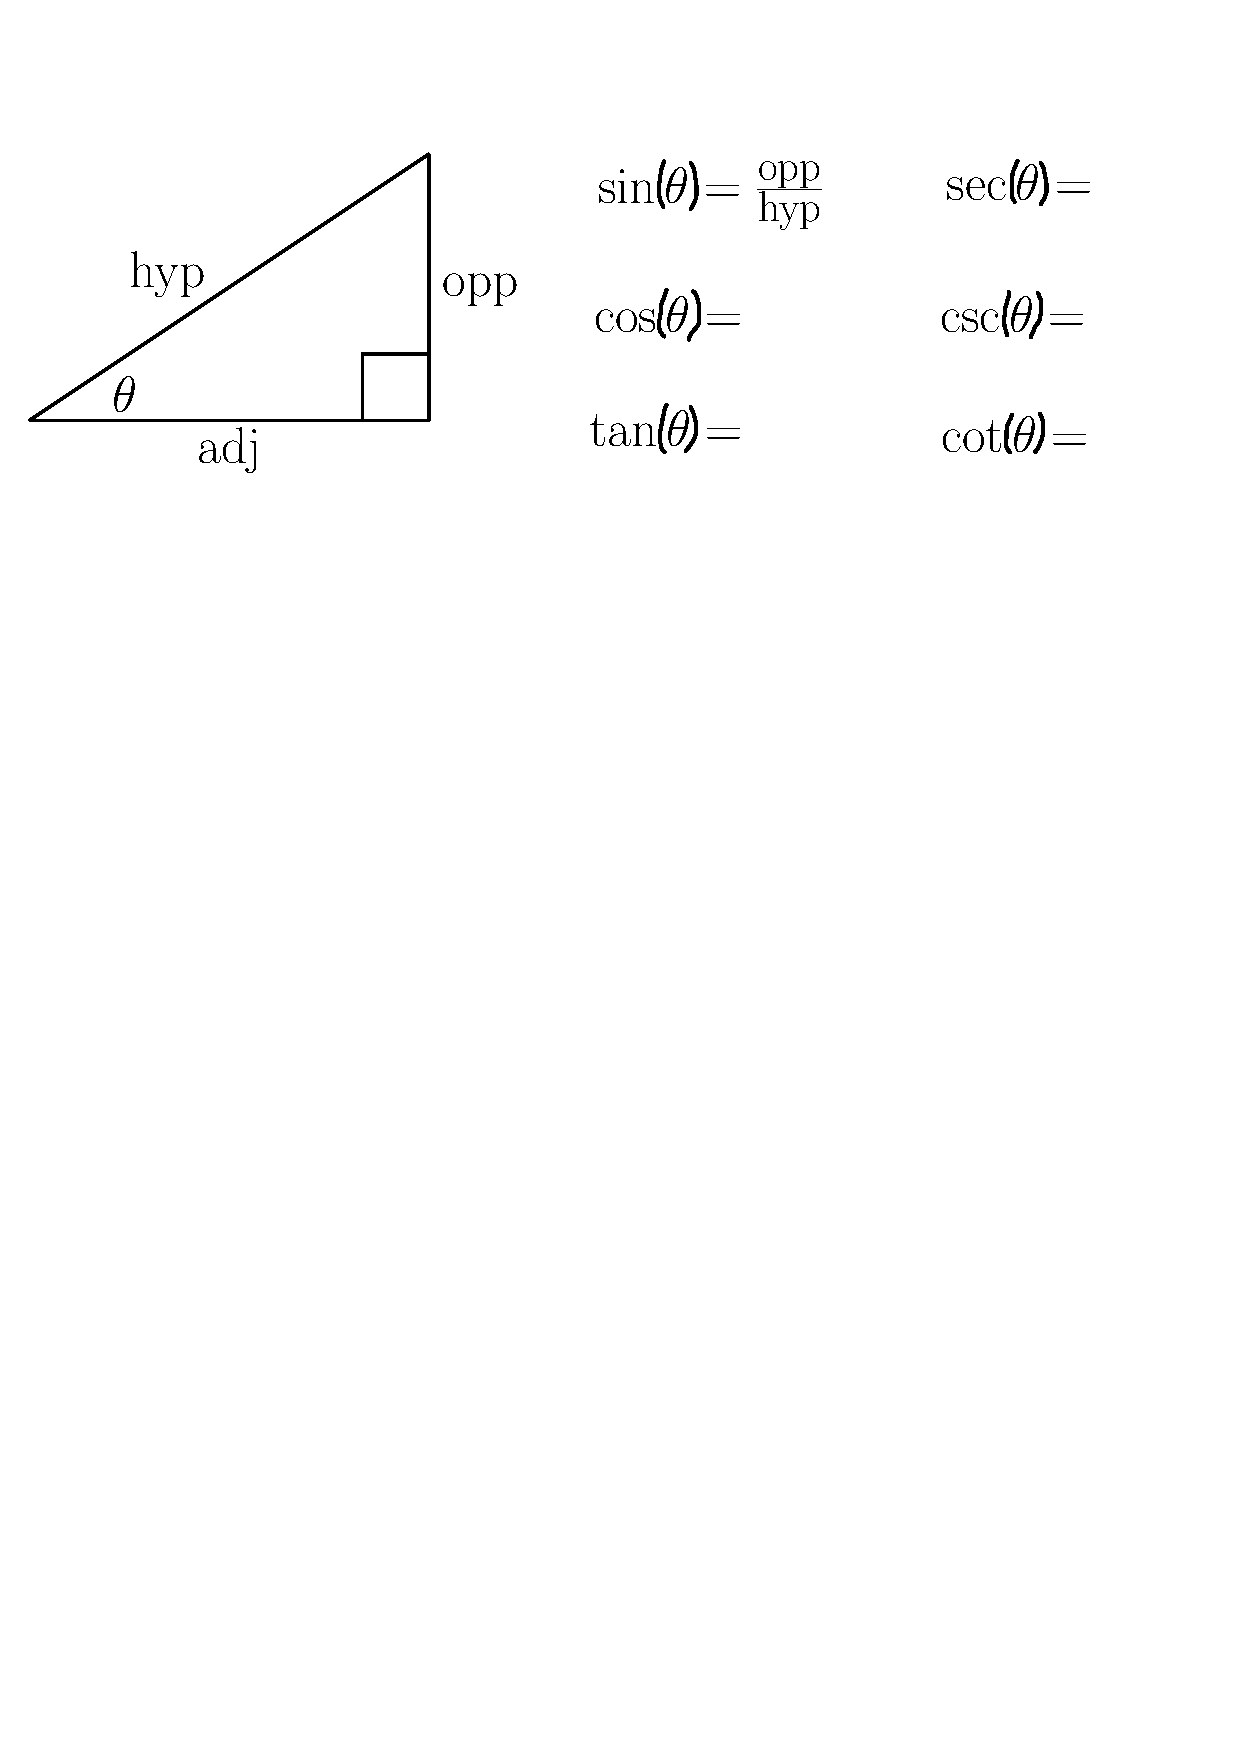
\includegraphics[scale=.5]{right_triangle.pdf} 

%\bigskip
\item $\displaystyle\int\frac{x^2}{\sqrt{x-5}} \  dx$
\vfill
\item $\displaystyle\int  \displaystyle\mathrm{cos}(\sqrt{x}) \ dx$.
\vfill


\pagebreak
\item $\displaystyle\int  \displaystyle\frac{1}{e^{3x}-e^x} \ dx$
\vfill
\item Evaluate  $\displaystyle\int  \displaystyle\mathrm{cos}(2x) \sqrt{1+\mathrm{sin}^2(2x)} \ dx$. \\
\textit{Hint: You may use that $\int \sec^3(x)dx = \frac{1}{2}\left(sec(x)tan(x)+\ln|sec(x)+tan(x)|\right)+C$}
\vfill
\iffalse
\begin{align*}
    \displaystyle\int  \displaystyle\mathrm{cos}(2x) \sqrt{1+\mathrm{sin}^2(2x)} \ dx &= \frac{1}{2}\displaystyle\int  \displaystyle \sqrt{1+u^2} \ dx \\
    &\hspace{1in} u= sin(2x), \; du/2 = cos(2x)dx\\
    &= \frac{1}{2}\displaystyle\int  \displaystyle \sqrt{1+tan^2(y)} \ sec^2(y)dy \\
    &\hspace{1in} u= tan(y), \; du = sec^2(y)dy\\
    &= \frac{1}{2}\displaystyle\int  \displaystyle \ sec^3(y)dy \\
    &= \frac{1}{4}tan(y)sec(y)+\frac{1}{4}ln|sec(x)+tan(x)|+C\\
    &= \frac{1}{4}u\sqrt{u^2+1}+\frac{1}{4}ln|\sqrt{u^2+1}+u|+C\\
    &= \frac{1}{4}sin(2x)\sqrt{sin^2(2x)^2+1}+\frac{1}{4}ln|\sqrt{sin^2(2x)+1}+sin(2x)|+C\\
\end{align*}
% (1/3) (sqrt(1+sin^2(2x))sin(2x))-(2/3)ln|sqrt{1+sin^2(2x)}+sin(2x)|+C 
Now.
\begin{align*}
    \frac{1}{2}\displaystyle\int  \displaystyle \ sec^3(y)dy&= \frac{1}{2}\left(tan(y)sec(y)-\displaystyle\int  \displaystyle \ tan^2(y)sec(y)dy \right)\\
    &\hspace{1in} v= sec(y), \; dw = sec^2(y)dy\\    
    &\hspace{1in} dv= sec(y)tan(y)dy, \; w = tan(y)\\ 
    &= \frac{1}{2}\left(tan(y)sec(y)-\displaystyle\int  \displaystyle \ (sec^2(y)-1)sec(y)dy \right)\\
    &= \frac{1}{2}tan(y)sec(y)-+\frac{1}{2}\displaystyle\int  \displaystyle \sec(y)dy-\frac{1}{2}\displaystyle\int  \displaystyle \ sec^3(y) dx  \\
    &= \frac{1}{2}tan(y)sec(y)+\frac{1}{2}ln|sec(x)+tan(x)|-\frac{1}{2}\displaystyle\int  \displaystyle \ sec^3(y) dx  \\
\end{align*}
So 
\[\frac{1}{2}\displaystyle\int  \displaystyle \ sec^3(y) dx =  \frac{1}{4}tan(y)sec(y)+\frac{1}{4}ln|sec(x)+tan(x)|+C\]
\fi

\end{enumerate} 

\end{document}
